%% Results note — self-contained proto-article, English draft (from the French revision of 17 September 2026).
%% English translation of note.tex — mechanical build derived from the same figures and numbers.
%% numbers_en.tex is regenerated from numbers.tex by scripts/make_numbers_en.py (decimal point only).
%% THIS IS A WORK IN PROGRESS TRANSLATION — see the notice below. Not for citation.
\documentclass[10pt,a4paper]{article}
\usepackage[T1]{fontenc}
\usepackage[utf8]{inputenc}
\usepackage[english]{babel}
\usepackage{lmodern}
\usepackage{amsmath,amssymb}
\usepackage[margin=2cm]{geometry}
\usepackage{booktabs,tabularx,array,longtable}
\usepackage{enumitem}
\usepackage{graphicx}
\usepackage{xcolor}
\usepackage{microtype}
\usepackage{float}
\usepackage[hyphens]{url}
\usepackage{hyperref}
\usepackage{caption}
\usepackage{tikz}
\usetikzlibrary{arrows.meta,positioning}
\usepackage{placeins}
\usepackage{fancyhdr}

\DeclareUnicodeCharacter{202F}{\,}
\hypersetup{colorlinks=true,linkcolor=blue!45!black,urlcolor=blue!45!black,
  pdftitle={[WORK IN PROGRESS] Rebound effect, emergence and steering in a physical model of a credit society},
  pdfauthor={Anatole Joseph-Stouls}}

\setlist{nosep}
\captionsetup{font=small,labelfont=bf}
\newcommand{\code}[1]{\texttt{#1}}
\newcommand{\chemin}[1]{\texttt{\path{#1}}}
\graphicspath{{figures/}}
\newcommand{\figurine}[3]{%
  \begin{figure}[htbp]\centering
  \includegraphics[width=#2\linewidth]{#1}
  \caption{#3}\label{fig:#1}
  \end{figure}}
\input{numbers_en}

\pagestyle{fancy}
\fancyhf{}
\renewcommand{\headrulewidth}{0.4pt}
\fancyhead[C]{\small\itshape Draft --- work in progress, not for citation --- English translation of a French working paper}
\fancyfoot[C]{\thepage}

\title{\vspace{-1.2cm}Rebound effect, emergence and steering\\[2pt]
in a physical model of a credit society}
\author{Anatole Joseph-Stouls\\
\small LIED --- Laboratoire interdisciplinaire des \'energies de demain\\
\small (Interdisciplinary Laboratory for Tomorrow's Energies)\\
\small \texttt{anatole.joseph-stouls@ens-rennes.fr}}
\date{}

\begin{document}
\maketitle
\vspace{-0.3cm}

\begin{center}
\fbox{\begin{minipage}{0.92\linewidth}\small\centering
\textbf{Work in progress --- draft translation.} This is an English
translation of a French working paper still under active revision. It
is shared for early feedback and discussion only, and should not be
cited or treated as a finished result. Figure axis labels and legends
are still in French pending regeneration in a later revision; the
mapping of the figure content is given in the glossary
(section~\ref{sec:glossaire}) and in the body text. The authoritative,
up-to-date version is the French original.
\end{minipage}}
\end{center}

\vspace{0.3cm}
\begin{abstract}\small
A local technical improvement does not necessarily translate into a
proportional response of the whole system. This work explores the
hypothesis that part of the rebound effect might stem from the
organization of exchanges, and not only from a change in behavior. We
build a physical toy model: entities extract a resource, lend each
other productive stock and can disappear, transmitting their losses to
their creditors. Population, network and inequality form during the
simulation; they are not fixed as targets.

The work articulates three questions: which regularities emerge, which
parameters allow them to be varied, and how the system responds to an
improvement in its technology. The simulations produce cascades of
varied sizes and long-tailed distributions of balance and interest.
Power-law fits with cutoff for cascade sizes leave systematic
deviations; self-organized criticality is not established. Contractions
of activity are short, with a decay of durations close to exponential.
The intensity of exchanges acts on propagation and tail statistics;
changing the time step does not reduce to a change of unit.

In the main configuration, increasing the extraction coefficient by
50\,\% increases aggregate production by about 35\,\%, not 50\,\%:
individual production increases while population decreases. The
response depends notably on the size of new entities relative to the
productive scale. These results establish an endogenous
non-proportionality in the model, not a calibrated measure of the real
energy rebound.
\end{abstract}

\section{Introduction: the internship's physical question}
The rebound effect denotes the fact that an improvement in energy
efficiency does not produce a proportional decrease in consumption. A
usual explanation is behavioral: the service becoming cheaper, one
consumes more of it. We explore here a different hypothesis, suggested
by work on urban metabolism \cite{hendrick} and by the application of
self-organized criticality to the economics of production \cite{bak}:
\emph{what if part of the response were endogenous to the organization
of exchanges}, that is a property of the way agents are coupled rather
than a sum of individual decisions?

This question calls for a model in which individual capacities can be
modified during the simulation and the ensuing reorganization observed,
without a rule having been written to produce a rebound. We build a
toy model to this end. It has no prices, no labor, no final
consumption, no households distinct from firms: it codes local
interactions and lets macroscopic regularities emerge.

Two objectives guide its construction: obtaining a collective response
that is not proportional to a microscopic change, and letting classes
of distributions emerge that can be confronted, with the necessary
precautions, with those observed in the economy. The guiding hypothesis
is that an organization exhibiting tendencies toward criticality might
amplify or dampen a local perturbation. In a self-organized critical
system, activity would spontaneously maintain itself near a propagation
threshold; a wide range of event sizes would be an indication of this,
not a proof. We do not assume this hypothesis to hold for the model
built here.

The stake of the internship is thus not only the last productivity
experiment. It includes building a coherent model, searching for
relevant endogenous variables, mapping sensitivities, and then running
controlled interventions. The reader first meets a four-entity example,
before the equations (\S\ref{sec:modele}). The protocol distinguishes
families of experiments (\S\ref{sec:protocole}). We then examine
emergence (\S\ref{sec:systeme}), steering and scales
(\S\ref{sec:pilotage}), and then the technological response and its
distribution (\S\ref{sec:rebond}). Secondary diagnostics and their
limitations are developed in the appendix.

\section{A minimal physical and accounting model}\label{sec:modele}
\subsection{Building intuition with four entities}
Imagine four entities able to extract a resource from their
environment. Each has a mobilizable stock $K_i$: the larger it is,
the more it extracts, but each additional unit of stock yields less
than the previous one. The function $f_i(K)=A_iK^{\gamma_i}$
describes this \emph{extraction technology}. The input joins the
stock, a fraction of which decays at each step. New entities appear
with the same endowment $K^\circ$ and, in the reference regime,
the same production exponent $\gamma^\circ=1/2$.

A well-endowed entity can lend stock to another, where that stock
produces more at the margin. This real transfer simultaneously
creates a claim for the lender and a debt for the borrower. The
\emph{principal} $q$ is the nominal amount recorded; the \emph{interest
service} $rq$ is the payment due at each step. Interest moves the
resource between entities, without creating any. The principal is not
progressively repaid in this model: this is a strong institutional
assumption.

\begin{figure}[htbp]\centering
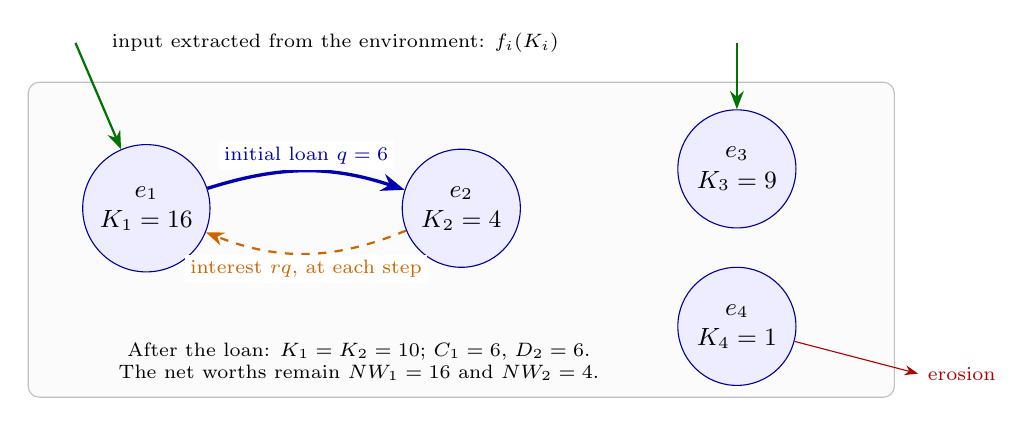
\begin{tikzpicture}[>=Stealth,font=\small,
 ent/.style={circle,draw=blue!60!black,fill=blue!7,minimum size=15mm,align=center},
 lab/.style={font=\scriptsize,fill=white,inner sep=2pt}]
\draw[rounded corners,fill=gray!3,draw=gray!50] (-1.5,-1.7) rectangle (9.5,2.3);
\node[ent] (a) at (0,0.7) {$e_1$\\$K_1=16$};
\node[ent] (b) at (4,0.7) {$e_2$\\$K_2=4$};
\node[ent] (c) at (7.5,1.2) {$e_3$\\$K_3=9$};
\node[ent] (d) at (7.5,-0.8) {$e_4$\\$K_4=1$};
\draw[->,very thick,blue!70!black] (a) to[bend left=18]
 node[lab,above] {initial loan $q=6$} (b);
\draw[->,dashed,thick,orange!80!black] (b) to[bend left=22]
 node[lab,below] {interest $rq$, at each step} (a);
\draw[->,green!45!black,thick] (-.9,2.8)--(a);
\node[lab] at (2.4,2.8) {input extracted from the environment: $f_i(K_i)$};
\draw[->,green!45!black,thick] (7.5,2.8)--(c);
\draw[->,red!70!black] (d)--(9.8,-1.4) node[right,font=\scriptsize] {erosion};
\node[align=center,font=\scriptsize] at (2.7,-1.25)
 {After the loan: $K_1=K_2=10$; $C_1=6$, $D_2=6$.\\
 The net worths remain $NW_1=16$ and $NW_2=4$.};
\end{tikzpicture}
\caption{\textbf{Real stock and accounting commitment are not the same thing.}
Fictitious example, inspired by the pedagogical diagram of the internship
presentation. The initial values are chosen to explain the mechanism, not
extracted from a simulation. Entities 3 and 4 show that not all entities
have to take part in the same exchange. Inputs and erosion are drawn on
only a few entities to lighten the diagram; the rules apply to all.
The external reservoir is not simulated.}
\label{fig:exemple}
\end{figure}

The loan thus preserves the instantaneous net worth of each partner,
but changes its productive capacity and its future commitments. An
entity may later be unable to honor its service, or owe more than it
holds. Its disappearance wipes out the claims held on it: its lenders
can in turn become insolvent. The coupling between real stocks,
persistent commitments and propagated losses is the mechanism studied
here.


\subsection{State, accounting, invariants}

The population is open and comprises a single type of agent, called an
\emph{entity}. No role -- lender, borrower, bank -- is declared;
all entities follow the same rules, and any observed differentiation
is emergent.

The variables $K_i,C_i,D_i,NW_i$, age and flows received or paid are
specific to entity $i$. The parameters $\lambda,\delta,\sigma,\rho$ and
the credit institution are common to the whole population.\footnote{The
parameters $\lambda$, $\delta$ and $\sigma$ are made explicit in
\S\ref{sec:pas}; $\rho$ and the credit institution in \S\ref{sec:credit}.
The glossary in appendix~\ref{sec:glossaire} gathers the notations.} The technology
$(A_i,\gamma_i)$ is attached to each entity; it is identical for all
at the reference point, but can differ after a targeted intervention.

An entity $i$ holds a real productive stock $K_i \ge 0$, counted in
joules, which we call its \emph{capital}. This is its intrinsic
productive size, not an accounting capital. A loan contract ties a
lender to a borrower through a nominal \emph{principal} $q > 0$ and a
per-step \emph{rate} $r > 0$. Summing over the contracts in which $i$
is involved gives its claims $C_i$ and its debts $D_i$, then its
\emph{net worth}
\begin{equation}
NW_i = K_i + C_i - D_i .
\label{eq:nw}
\end{equation}

The asymmetry between the two stocks is constitutive: capital is real,
productive and depreciable, whereas the principal is nominal, perpetual
and not amortized. The debt network can therefore remain heavy while
real assets erode.

The rules algebraically enforce, at every step, $K_i \ge 0$,
$\sum_i C_i = \sum_i D_i$, the equality between the sum of the net
worths of the survivors and their total capital, and the real balance
sheet
\begin{equation}
\sum_i K_i(t{+}1) - \sum_i K_i(t) = \text{endowments} + \text{shock}
  + \text{production} - \text{depreciation} - \text{destruction},
\label{eq:bilan}
\end{equation}
the five terms on the right being recorded separately at each step.
The numerical check accounts for floating-point rounding.
Loans and interest are purely internal transfers: there is neither
creation nor leakage of joules outside the channels named
in~\eqref{eq:bilan}.

\subsection{A time step}\label{sec:pas}

The phases run in this order, which is part of the model.
Scheduled interventions are applied before births.

\begin{enumerate}[label=(\roman*),leftmargin=2.2em]
\item \textbf{Births.} A number $B_t \sim \mathrm{Poisson}(\lambda)$
  of entities enters, each endowed with a capital $K^\circ$. The parameter $\lambda$ is
  the \emph{birth intensity} and $K^\circ$ the \emph{birth endowment}.
\item \textbf{Shock.} $K_i \leftarrow K_i \, e^{\eta_i}$, with
  $\eta_i \sim \mathcal{N}(-\sigma^2/2,\ \sigma^2)$ independent. The
  multiplicative mean equals one: no drift is imposed. The parameter
  $\sigma$ fixes the common amplitude of the noise; the draw $\eta_i$ is
  individual and renewed at each step. This is not a shared global
  shock.
\item \textbf{Production.} $K_i \leftarrow K_i + A\,K_i^{\gamma}$, with
  $0<\gamma<1$. The parameter $A$ is the \emph{productivity} of the
  technology and $\gamma$ its \emph{production exponent}. Concavity is
  essential: it is what creates a gain from pooling
  (\S\ref{sec:credit}).
\item \textbf{Interest service.} This is the periodic payment of the
  loan charge, without repayment of the principal. Each borrower pays
  $\sum r q$ drawn from its capital; if it cannot, it pays pro rata and
  enters service default.
\item \textbf{Depreciation.} $K_i \leftarrow (1-\delta)K_i$, where
  $\delta$ is the \emph{per-step depreciation rate}. It represents the
  temporal erosion of the stock; its value therefore depends on the
  duration chosen for a step (\S\ref{sec:temps}). Principals, for their
  part, do not depreciate.
\item \textbf{Market.} See \S\ref{sec:credit}.
\item \textbf{Bankruptcies.} See \S\ref{sec:faillite}.
\item \textbf{Measurements.} No logging option consumes a random draw:
  trajectories with and without measurement are identical.
\end{enumerate}

\subsection{Stocks, flows and the physics--economics correspondence}
\label{sec:physique}
The parallel between physics and economics is the center of the
approach, not an analogy added after the fact. It is nonetheless
necessary to distinguish a correspondence of dimensions, a
representational hypothesis and an empirical validation.
The model is a fundamental study of interactions: the entity remains
generic, and can shed light on a concrete system if the relevant
mechanisms are indeed present there, without implicitly becoming a
person and then a firm.

\begin{center}
\begin{tabularx}{\linewidth}{@{}lXX@{}}
\toprule
Object & Dimension and operation & Proposed economic reading \\
\midrule
$K_i$ & Stock, in model joules & Mobilizable productive size \\
$A_iK_i^{\gamma_i}$ & Production added during a step, in joules & Productive flow, not a wage \\
$A_iK_i^{\gamma_i}/\Delta t$ & Mean power over a step & Production capacity per unit of time \\
$q$ & Nominal principal, same unit of account as $K$ & Claim and debt, not amortized \\
$rq$ & Transfer during a step & Interest service, not resource creation \\
$NW_i$ & Accounting stock $K_i+C_i-D_i$ & Balance-sheet position, distinct from the physical stock \\
\bottomrule
\end{tabularx}
\end{center}
A watt is one joule per second. The engine's outputs are in joules
\emph{per step}; calling them watts would require fixing $\Delta t$ in
seconds, which has not been calibrated.\footnote{In the update
$K\leftarrow K+A K^\gamma$, $A$ has dimension
$\mathrm{J}^{1-\gamma}$ for the production of one step. The
coefficient of a corresponding differential equation would have
dimension $\mathrm{J}^{1-\gamma}/\mathrm{s}$. Comparing them without
specifying the step would make a physical dimension disappear. The
rate $r$ is a fraction due per step; $r/\Delta t$ has the inverse
dimension of a time.}

The interpretive hypothesis is that certain monetary transfers
represent transfers of entitlements to mobilize exergy. The real stock
and the nominal network are thus coupled, but not identical: a loan
moves $K$ and simultaneously records a claim and a debt. Production
represents an input to the modeled stock; the external reservoir that
enables it is not described. The internal balance sheet is closed in
accounting terms, not thermodynamically over the whole
economy--environment system. Furthermore, the observable called
"total income" is $\mathrm{prod}+\mathrm{int\_in}$: it adds
production and transfers received, and must not be equated without
correction to an aggregate net production.

\subsection{Scales: which parameters are truly independent?}
\label{sec:parametres_reduits}
In the homogeneous regime, without noise or credit, the order
production then depreciation gives
\[
 K_{t+1}=(K_t+A K_t^\gamma)(1-\delta),\qquad
 K_{\rm aut}=\left[\frac{A(1-\delta)}{\delta}\right]^{1/(1-\gamma)}
\]
for $A>0$, $0<\delta<1$ and $0<\gamma<1$. $K_{\rm aut}$ is the stock toward which an isolated entity, without
credit or noise, tends when extraction and depreciation offset each
other. This deterministic fixed point is not a mean of the noisy
system. Setting $x_i=K_i/K_{\rm aut}$ transforms
production into
\[
 x_i\longleftarrow x_i+\frac{\delta}{1-\delta}x_i^\gamma .
\]
At fixed institution, the common scale of $A$ and $K^\circ$ can thus
be replaced by the ratio $\kappa^\circ=K^\circ/K_{\rm aut}$: it
measures the size of a new entity relative to what it could reach
alone. A low value means it enters far below this scale. For a
toy model, avoiding double-counting the same scale freedom is
essential.\footnote{An equivalent option is to choose $K^\circ$ as the
unit and to retain $a=A (K^\circ)^{\gamma-1}$. The point here is to
eliminate \emph{one} unit-of-capital freedom, not to show that the
other parameters are redundant: $\gamma$, $\delta$, $\sigma$,
$\lambda$ and the institution remain relevant. An invariance of
certain statistics with respect to $\lambda$ is not a trajectorial
equivalence of populations of different sizes.}

The rescaling $K,q,K^\circ\mapsto c(K,q,K^\circ)$ and
$A\mapsto c^{1-\gamma}A$ preserves the homogeneous equations and the
marginal rates. Absolute numerical thresholds and the engine's
rounding limit software exactness; recalibrating the time step is not
an exact symmetry of the discrete market: the numerical study is
presented in \S\ref{sec:temps} and the non-equivalence of the
operations is detailed in appendix~\ref{sec:composition_temps}. A rise
in $A$ at fixed $K^\circ$ therefore changes $\kappa^\circ$, whereas its
compensation $K^\circ\mapsto K^\circ\,m^{1/(1-\gamma)}$ preserves it.
The two are distinct experiments: compensation is a control, not an
imposed physical correction.

The tension $T=K_{\rm aut}/K_{\rm eq}$, with
$K_{\rm eq}=(Y/(N_{\rm prod}A))^{1/\gamma}$, compares the individual
scale without credit to the observed productive scale. Here $Y$ is
the total production of a step and $N_{\rm prod}$ the number of
entities present in the productive phase, which can differ from the
surviving headcount at the end of the step. $K_{\rm eq}$ is the
fictitious stock that would give a representative entity the mean
production $Y/N_{\rm prod}$; for $\gamma\ne1$, this is not the mean
stock. A large $T$ therefore indicates a productively equivalent
stock far below the autarkic scale. This tension is useful in
particular at fixed $\delta$; it is neither a universal state
variable, nor another name for the whole
credit--mortality--population chain.

The coupling of distinct physical and economic spheres joins an
existing thermodynamic motivation \cite{herbert}, without reusing its
model or identifying money with exergy.

\subsection{Credit as cooperation, and the rate as sharing}
\label{sec:credit}

For two entities with the same concave technology, the marginal return
$f'(K)=A\gamma K^{\gamma-1}$ is larger for the less endowed one.
A transfer toward it therefore increases \emph{joint} production as
long as it does not exceed the equalization of marginal returns. This
result does not hold for any amount nor for any heterogeneous pair. It
is the sole motive for credit in this model: there is neither
anticipation, nor time preference, nor price.

Figure~\ref{fig:art_technologie} illustrates the role of technology and
the gain from lending. At fixed $\gamma$, $A$ multiplies extraction per
step; on its own it is not a power in watts. The exponent $\gamma$
measures individual returns to scale. Between zero and one, it makes
the function concave and allows a reallocation gain: calling it
directly a "propensity to collaborate" would be excessive. At
$\gamma=1$ and identical technology, this gain disappears; its
variation with $\gamma$ requires fixing the units and the states
compared.

\figurine{art_technologie}{1.0}{\textbf{Technology and cooperation gain.}
On the left, the technologies $f_1(K)=2K^{1/4}$ and $f_2(K)=K^{1/2}$
cross at $K=16$, for a production of 4 per step; the initial stocks
are distinct, $(K_1,K_2)=(20,4)$. The coefficients are expressed in a
single fixed stock unit. On the right, a loan of 1 toward 2 increases
joint production up to the equalization of marginal returns. The area
between gain and loss measures the joint surplus; the crossing of the
productions on the left is not this equalization.
These curves are analytical, at fixed states, without a statistical
interval.}

The market phase carries out $\lfloor\rho n\rfloor$ rounds for an
eligible pool of $n$ entities in the configurations studied; $\rho$ is
the market intensity (default value $1$). Encounters are pairwise.
The amount targets the equalization of marginal returns in the main
configuration. The free direction of the loan recovers the rich-to-poor
transfer in the homogeneous regime, not necessarily in the
heterogeneous regime.

There is therefore a \emph{cooperation surplus} to be shared, and the
interest rate is the sharing mechanism. For a contract of principal
$q$, let $L$ denote the production loss suffered by the giver by
parting with this stock, and $\Delta$ the joint production gain of the
pair -- the surplus. The service paid per step then decomposes as
\begin{equation}
r\,q \;=\; L \;+\; p\,\Delta.
\label{eq:partage}
\end{equation}
The number $p$ is the \emph{sharing}. The imposed \texttt{bargain} rule
explores $p\in[0,1]$; the implicit sharing of another rule can exceed
these bounds. At $p = 0$, the service exactly compensates the
productive loss computed at contract creation; the receiver keeps the
surplus. At $p = 1$, the lender also receives all of this surplus.
This instantaneous comparison does not guarantee the contract's
balance over its lifetime. Equation~\eqref{eq:partage} \emph{defines}
$p$ for any rate rule, which makes it possible to place a given rule on
the sharing scale -- this is what we exploit in
\S\ref{sec:partage}. The reference rule, used by default, sets $r$ to
the geometric mean of the marginal returns of the two entities.

\subsection{Bankruptcy and cascade}
\label{sec:faillite}

An entity goes bankrupt if it is in service default or if $NW_i < 0$.
The rule is deliberately brutal: its contracts are \emph{cancelled} --
its creditors lose the principal, with no recovery or buffer -- and its
residual capital is \emph{destroyed}. A default therefore directly
annihilates assets held by others and can render them insolvent in
turn; the new insolvencies form the next generation, and iteration
continues to the fixed point \emph{within the same step}.

This rule is what distinguishes a contagion from mere synchronization.
When a borrower dies, each lender loses the corresponding principal,
which defines a directed edge from the dead entity to the lender. An
\emph{avalanche} is a weakly connected component of this loss graph,
restricted to entities that died in the same step.
\begin{figure}[htbp]\centering
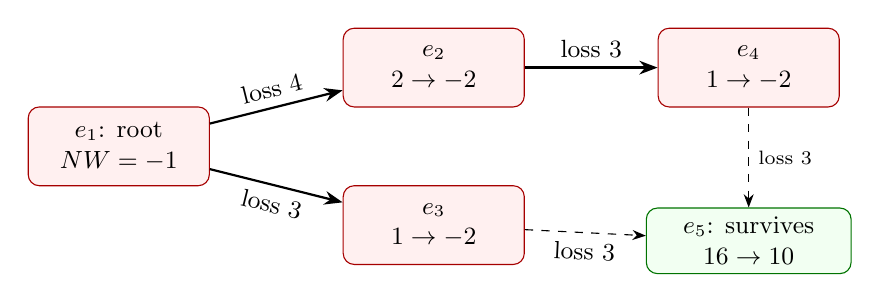
\begin{tikzpicture}[>=Stealth,font=\small,
 dead/.style={draw=red!65!black,fill=red!6,rounded corners,align=center,minimum width=23mm,minimum height=10mm},
 safe/.style={draw=green!45!black,fill=green!5,rounded corners,align=center,minimum width=26mm}]
\node[dead] (a) at (0,0) {$e_1$: root\\$NW=-1$};
\node[dead] (b) at (4,1) {$e_2$\\$2\to-2$};
\node[dead] (c) at (4,-1) {$e_3$\\$1\to-2$};
\node[dead] (d) at (8,1) {$e_4$\\$1\to-2$};
\node[safe] (e) at (8,-1.2) {$e_5$: survives\\$16\to10$};
\draw[->,thick] (a)--node[above,sloped] {loss $4$} (b);
\draw[->,thick] (a)--node[below,sloped] {loss $3$} (c);
\draw[->,thick] (b)--node[above] {loss $3$} (d);
\draw[->,dashed] (c)--node[below,sloped] {loss $3$} (e);
\draw[->,dashed] (d)--node[right,font=\scriptsize] {loss $3$} (e);
\end{tikzpicture}
\caption{\textbf{A directed propagation tree, not the direction of the loan.}
Example that is accounting-feasible with five entities. Before resolution,
their stocks are worth $(6,1,1,1,10)$; the loans are
$e_2\to e_1:4$, $e_3\to e_1:3$, $e_4\to e_2:3$,
$e_5\to e_3:3$ and $e_5\to e_4:3$.
The arrows in the diagram go, conversely, from the defaulting borrower to
the affected creditor. The component of the four deaths has one root and
two generations of propagation: $S=4$, $b_1=b_2=3/4$.
The losses suffered by $e_5$, a survivor, do not make it part of
the avalanche of deaths. The general model allows several parents,
unlike this tree-shaped example.}
\label{fig:cascade}
\end{figure}


Two propagation measures follow: the \emph{branching ratio}
$b_1 = 1 - (\text{roots}/\text{deaths})$, where a root is a bankruptcy
that entered directly in the step's initial queue, and the \emph{mean
offspring} $b_2$, the mean number of causal pairs between successive
generations per death. The two coincide
if and only if every non-root death has exactly one parent; their gap
measures the excess of edges per death:
$b_2-b_1=\sum_v(d_v-1)/N$,
with $d_v$ the number of previous-generation parents of a non-root and
$N$ the total number of deaths. This is neither the proportion of
victims with several parents, nor the number of individually
sufficient causes.


\section{Experimental approaches in several steps}\label{sec:protocole}
The first step is a \emph{mapping}: varying parameters to distinguish
robust regularities from effects specific to a given configuration. The
M4B study explores births, stock erosion, noise, endowment and the size
of the encounter pool. It includes one-parameter-at-a-time variations,
a global plan of 64 points with three seeds, two-parameter cuts and a
confirmation with five new seeds. Its inventory counts 594 simulations,
not all of whose results are reproduced here. The confirmation center is
$\lambda=30$, $\delta=0.05$, $\sigma=0.25$, $K^\circ=25$, $k=3$, $A=1$,
$\gamma=1/2$.

The second step is \emph{scale identification}: determining what
amounts to a freedom of unit and what actually changes the exchanges.
Time-rescaling trials use three seeds per configuration, with durations
brought back to a common unit. They are presented separately, since
their protocol is not that of the technological interventions.

The third step is the \emph{paired intervention}. At the main point,
$\lambda=30$, $K^\circ=25$, $\sigma=\delta=0.01$, $A=1$, $\gamma=1/2$,
$\rho=1$ and $k=2$. The population numbers about 1132 entities in the
observed regime. Twelve states are seeded up to step 2000; each yields
a control and variants, with the same initial state and the same
generator at the branch point. Individual draws can then diverge with
the population sizes. The M4.4 campaign comprises 372 inventoried
simulations, not 372 independent repetitions of a single experiment.

The M4B results and those of the main configuration are not
interchangeable: beyond noise and depreciation, M4B uses a pool of $k$
entities and a geometric target, while the main configuration uses
pairwise encounters and a marginal-equalization target. Each figure
states its family, its window and its number of seeds. Engine names
serve to trace sources, not to replace these scientific definitions.

The variation of $k$ belongs to the historical M4B exploration; the
later main experiments fix encounters at $k=2$. This choice removes $k$
from the levers of this configuration, without retroactively modifying
the parameters of the earlier experiments. Software extensions have
undergone compatibility checks in specified regimes; this does not make
different market rules equivalent. Appendix~\ref{sec:compatibilite}
distinguishes these checks from changes to the model.

A seed, not an entity or a step, constitutes the unit of repetition.
Unless stated otherwise, levels are averaged over $3000<t\le4000$, then
ratios are computed seed by seed. A 95\% CI bar is a Student interval
between these repetitions. A drift diagnostic compares the first and
last quarters of the window; its formula, its results and its limited
scope are given in Appendix~\ref{sec:stationnarite}. The absence of a
detected mean drift does not demonstrate strict stationarity.

\section{What emerges without being imposed}\label{sec:systeme}
\subsection{A renewed population and a credit network}
The rules fix the mean flow of births, not the population size, the
lifetime or the lender/borrower roles. In the configurations retained,
the series settle into a fluctuating regime with no observed unbounded
growth. Entries balance exits on average, but a stable age distribution
does not imply that any particular entity is at equilibrium. New
entities grow, incur commitments and disappear at varied ages.

Little's law relates, under a stable regime and with controlled
temporal boundaries, the mean population to the entry flow multiplied
by the mean lifetime. It is a demographic identity useful for
organizing measurements, not an explanation of the lifetime. The
lifetime depends on noise, the network and the bankruptcy rules. The
deterministic equilibrium of an isolated entity does not by itself
predict the collective state.

\subsection{Directed cascades and a wide range of sizes}
The loss graph makes it possible to distinguish propagation from
temporal coincidence. The example in Figure~\ref{fig:cascade} gives the
definition; the distributions in Figure~\ref{fig:art_avalanches} show
the simulated realizations. We fit, on each seed, a discrete
probability
\begin{equation}
 P(S=s)=Z^{-1}s^{-\alpha}\exp(-s/S_c),\qquad s\ge1,
 \label{eq:avalanche}
\end{equation}
where $Z$ normalizes the sum of probabilities and $S_c$ describes a
soft cutoff, not an absolute maximum size. At the main control, the
twelve fits give $\alpha=1.623\pm0.009$ and $S_c=206\pm11$; under
$A\times1.5$, $\alpha=1.667\pm0.009$ and $S_c=185\pm7$. These
uncertainties describe the between-seed variability of this estimator.
They validate neither the chosen family nor the identification of the
cutoff with the system size.

\figurine{art_avalanches}{1.0}{\textbf{Histograms, fits and repetitions.}
M4.4, twelve seeds per condition, $3000<t\le4000$. Points give the
per-class probability divided by class width; bars are between-seed
95\% CIs. Curves are the means of the discrete cutoff-exponential fits,
ribbons a bootstrap of 2000 draws of whole runs. Dashed lines indicate
the reference slope $-\alpha$, not the complete truncated law. $R^2$
values are computed on the logarithms of non-empty classes, then
averaged across seeds. The left panel represents the control whose
individual exponents are repeated on the right; the central panel
represents the other series.
\textsuperscript{1}Bars too long for the log scale are truncated at
95\,\% of the level; their full values remain in the data.}

The cutoff model is fitted by likelihood on integer sizes, not by
selecting the straightest portion of the histogram. The mean $R^2$
values, about $0.938$ and $0.928$, do not constitute a test of Pareto
behavior. Despite these high values, the curves underestimate part of
the intermediate sizes and overestimate the extremes: the visible
deviations exceed several of the between-seed bars. The simple form of
Equation~\eqref{eq:avalanche} therefore does not account for the whole
distribution at the precision of the data. Choosing the cutoff to
simultaneously optimize a bootstrap variance and an $R^2$ would also
select favorable fluctuations; we retain here one stated model and
support, with the caveats of Appendix~\ref{sec:ajustements}.

At the main point, $b_1=\BUnControle\pm\BUnControleIC$ and
$b_2=\BDeuxControle$: some deaths have several parents. The fact that
$b_1<1$ is not, by itself, a test against criticality: its definition
as the fraction of propagated deaths bounds it by construction.
Conversely, an extended tail does not demonstrate SOC. Finite-size
study and the definition of events across several steps remain
necessary.

\subsection{Short contractions, distinct from avalanches}
An avalanche is a network event within a single step. A contraction is
a sequence of steps over which an aggregate quantity decreases. They
are therefore neither the same observation nor two definitions of the
same size. In the central M4B regime, the mean durations of stock and
production contractions are close to two steps.
Figure~\ref{fig:art_cycles} formalizes their decay by a discrete
exponential, $P(D\ge d)=\exp[-\beta(d-1)]$, $d=1,2,\ldots$.

\figurine{art_cycles}{1.0}{\textbf{Contraction durations: an exponential,
not an imposed power law.} Central M4B, five seeds 11--15,
$1000<t\le4000$, unsmoothed; stock and production are treated
separately. $\beta$ is estimated per seed from the mean duration. Points
are the empirical survival values and their 95\% CIs; curves average
the five fits. Descriptive $R^2$ values bear on the log-survival at
the observed durations, whose points are dependent. Logarithmic bars
are truncated according to the convention of
Figure~\ref{fig:art_avalanches}. Episodes touching a window boundary
are counted per the existing protocol; this is not a survival analysis
correcting for censoring.}

We find $\beta=0.731\pm0.029$ for stock and $0.696\pm0.035$ for
production, with mean log-survival $R^2$ close to $0.98$. Wright
\cite{wright} shows precisely why power law and exponential must be
compared over the whole set of durations, without discarding the
shortest episodes. His study covers annual GDP contractions of 17
economies between 1870 and 1994; our uncalibrated steps are not years.
The resemblance in shape motivates a future comparison; these short
contractions do not by themselves support a power law of durations nor
the SOC hypothesis.

\subsection{Balance and interest distributions: what plausibility?}
Net worth (denoted $NW$) is the model's quantity closest to a net
wealth: real assets plus claims minus debts. Interest received
constitutes a financial income flow. Their distributions emerge from
entities subject to the same rules, not from wealth classes imposed at
birth. In the main regime, the time-averaged Gini indices are close to
$0.613$ for net worth and $0.513$ for interest received.
Figure~\ref{fig:art_lorenz} represents distinct snapshots of these time
averages.

\figurine{art_lorenz}{1.0}{\textbf{The collective distribution persists
despite individual turnover.} M4.4 control, twelve seeds: Lorenz curves
at $t=2010$, $3000$ and $4000$, and between-seed 95\% CIs. Each
observable has its own ranking.}

To gauge orders of magnitude, the net-worth Gini of US households is
$0.852$ in the 2019 SCF \cite{fedgini}: the main model is thus
noticeably less unequal on this measure. The CBO reports a Gini of
$0.516$ for income before means-tested transfers and taxes in 2019
\cite{cbogini}. Its numerical closeness to $0.513$ does not validate the
model's distribution: interest received includes neither wages nor all
capital income, and our entities are not households weighted by size.
A direct confrontation requires the same type of actor, the same
period and the same accounting definition. We therefore do not compare
the Gini of physical stock to that of income to conclude on economic
plausibility.

The tails of net worth and interest are compatible with power-law fits
over part of the domain; their statistical identification remains open
\cite{clauset,wildauer}. A log-normal and a cutoff power law each have
two shape parameters at a fixed threshold. If the cutoff depends on
system size, that dependence must be estimated across several sizes; it
does not automatically remove a parameter from a fit performed at a
finite size. The existing tests and their limitations are detailed in
Appendix~\ref{sec:ajustements}.

\section{Steering: which levers change which properties?}\label{sec:pilotage}
\subsection{A hierarchy of sensitivities, not a single control knob}
The M4B mapping separates effects that would be confounded in a
comparison of only two trajectories. Noise $\sigma$ affects survival and
exposure; endowment $K^\circ$ changes the entry position of young
entities. Depreciation shifts the productive scale and also enters
balance sheets; the birth rate $\lambda$ allows exploring populations of
different sizes. These are tendencies within the domain studied, not
exclusive roles nor demonstrated independences.

\figurine{art_sensibilite}{0.72}{\textbf{Returning to the levers studied
during model construction.} M4B confirmation, five independent seeds
per cell, $T=4000$. Net-worth Gini computed on the final snapshot, not
the Gini of capital nor of the pool. The other parameters are those of
the historical M4B center, notably $k=3$; only $\sigma$ varies. The old
sweep of $k$ is not shown here, as the later main experiments fix
encounters at two entities. Bars are Student 95\% CIs recomputed from
the per-seed values.}

The finite-size variation is particularly important for the critical
hypothesis. In the M4B confirmation, as $\lambda$ goes from 10 to 30
then 100, the mean observed maximum avalanche size goes from 29 to 54
then 110. The fitted cutoffs do not all behave as regularly: at
$\lambda=100$, the estimated value is far beyond the sample, hence
poorly identified. These observations support a finite-size study; they
do not justify imposing a universal cutoff law or mixing the M4B and
M4.4 exponents.

\subsection{Encounter intensity as an experimental lever}
In the main configuration, $\rho$ sets the number of encounters per
step. Varying it from $0.5$ to $3$ allows measuring its response at
five levels, with twelve seeds per level. The fitted exponents of the
interest and net-worth tails, as well as branching, increase; the
net-worth Gini varies more weakly.

\figurine{art_rho}{0.95}{\textbf{Measuring steering on defined
observables.} M4.4, five values of $\rho$, twelve seeds,
$3000<t\le4000$. Exponents and branching are those of the per-seed
analyses; the net-worth Gini is recomputed on the panels of the same
window. Points: means and 95\% CIs. Curves: per-seed log-log fits;
slopes and $R^2$ are then averaged, with 95\% CIs of the slopes.}

The measured log-log slopes are $0.0465\pm0.0074$ for the interest
exponent, $0.0272\pm0.0074$ for the net-worth exponent and
$0.1345\pm0.0020$ for $b_1$. That of the net-worth Gini is
$-0.0084\pm0.0023$: a weak but detectable effect on average, which
should not be confused with the strong response of the pool's Gini. A
significant mean slope does not imply that every increment is monotone
within every seed. The result is a local steering lever, not a
universal law nor proof of a distribution family.

\subsection{Changing a scale is not always changing the system}
Non-dimensionalization (\S\ref{sec:parametres_reduits}) removes a
freedom of unit: multiplying all stocks and principals by $c$ and $A$
by $c^{1-\gamma}$ preserves the homogeneous equations. The quantity
$\kappa^\circ=K^\circ/K_{\rm aut}$ instead expresses a relative position
that changes the dynamics. At $\gamma=1/2$, multiplying $A$ by 1.5
multiplies $K_{\rm aut}$ by $2.25$; keeping $K^\circ$ fixed therefore
divides $\kappa^\circ$ by $2.25$.

This distinction organizes the experiments: a technical change at fixed
endowment tests a relative displacement of new entrants, while a
compensated endowment preserves that relative position. One must
further distinguish compensating only the births after an intervention
from rescaling \emph{the whole} initial state, including the nominal
network. Only the latter directly falls under the exact symmetry of
the equations.

\subsection{The granularity of the time step}\label{sec:temps}
Depreciation represents a temporal erosion. If a step lasts $\Delta t$
and the continuous erosion rate is $d$, then $\delta=1-e^{-d\Delta t}$.
Grouping $s$ steps therefore requires
\[
 \delta'=1-(1-\delta)^s,\qquad
 \sigma'=\sqrt{s}\,\sigma,\qquad \lambda'=s\lambda.
\]
The last two relations compose, respectively, independent log-normal
shocks and Poisson births \emph{in law}, for isolated phases. They do
not guarantee that the coupled system follows the same law. Per-step
flows must also be converted: $A'\simeq sA$ and $\rho'\simeq s\rho$; the
nominal service of existing contracts must be converted if one
transforms an already indebted state.

\figurine{art_temps}{1.0}{\textbf{Changing the step does not stop at
three substitutions.} Live-v1 experiments from an empty state, three
seeds per configuration. Common window $1200<t_{\rm ancien}\le2000$.
Flows of the grouped steps are divided by $s$, not the stocks. The
first three trials group two steps; the fourth groups four. The last
compares two configurations at $\delta=0.002$ before conversion, and
therefore has its own reference. Points: per-seed averaged ratios;
bars: Student 95\% CIs, wide with three repetitions.}

The simulations of Figure~\ref{fig:art_temps} leave a residual even
after converting all these coefficients. Two steps successively update
production, commitments, population and encounters; a single more
intense step does not reproduce this alternation. Reducing $\delta$
alone does not remove the residual in the trial performed. These
controls rule out a simple unit error as a complete explanation,
without isolating each compositional effect. A proper convergence study
would require jointly reducing all relevant increments and comparing at
a fixed physical horizon. It remains to be carried out.

\section{Collective response to a technological improvement}\label{sec:rebond}
\subsection{What changes and what the elasticity measures}
The main experiment multiplies $A$ by $m=1.5$ for all living entities
and for future births, starting at step 2001. At unchanged stock and
fixed exponent $\gamma$, each entity would produce exactly 50\,\% more:
this is the proportional reference. But stocks, the network and the
population size then evolve. We measure
\begin{equation}
 \varepsilon_s=\frac{\ln(\overline Y_{s,T}/\overline Y_{s,C})}{\ln(1.5)},
 \qquad \widehat\varepsilon=\frac1{12}\sum_{s=1}^{12}\varepsilon_s,
 \label{eq:eps}
\end{equation}
where $Y$ is total production, $T$ the treated arm, $C$ the control and
the overbar a mean over $3000<t\le4000$. The denominator is the
logarithm of the imposed technical factor, not a fitted constant. A
proportional response gives $\varepsilon=1$; $0<\varepsilon<1$ means a
sub-proportional increase; $\varepsilon<0$ would mean a decrease despite
the improvement. This is a \emph{finite} elasticity, not an
infinitesimal derivative.

\subsection{A positive but non-proportional response}
At fixed birth endowment, $\widehat\varepsilon=0.7473\pm0.0106$.
\textbf{The collective response is not proportional to the individual
improvement.} The representative factor $1.5^{0.7473}\simeq1.354$
corresponds to about 35\,\% additional production. The arithmetic mean
of the ratios is not exactly this transform of the mean of the
logarithms; the per-seed values are kept.

\figurine{art_reponse}{1.0}{\textbf{The same improvement, two birth
conventions.} M4.4, twelve paired seeds. Left, relative treated/control
gaps, smoothed over 101 steps per seed before computing the 95\% CIs.
Right, finite elasticities on $3000<t\le4000$; pale points: seeds;
bars: 95\% CIs. Compensation applies to births, $K^\circ\to2.25K^\circ$,
not to already-present stocks and contracts. The line at 2 is a
prediction of full-state symmetry, not a constraint imposed on this
fit.}

The end-of-step population contracts by about a quarter, while
production per entity increases. To keep an exact decomposition after
time averaging, one can define the mean population yield by
$\overline y=\overline Y/\overline N$. Then
$\ln(\overline Y_T/\overline Y_C)=
\ln(\overline N_T/\overline N_C)+\ln(\overline y_T/\overline y_C)$
by definition. $\overline y$ is not in general the time average of
$Y(t)/N(t)$; one must also distinguish the step's producers from the
end-of-step survivors. A decomposition identity does not constitute a
demonstration of the demographic mechanism.

If instead the endowment tracks the productive scale, the measure is
$2.0029\pm0.0148$. This value is compatible with $1/(1-\gamma)=2$, the
prediction of full homogeneous rescaling, but numerical compatibility
does not make the two protocols identical. Precisely, at $\delta=0.01$
and $\gamma=1/2$ fixed, $K_{\rm aut}$ goes from $9801$ to $22052.25$ when
$A$ goes from $1$ to $1.5$. At unchanged endowment $K^\circ=25$, the
ratio $\kappa^\circ$ goes from about $0.00255$ to $0.00113$: new
entities enter smaller relative to this scale. Compensation consists in
raising their endowment to $56.25$, in order to preserve $\kappa^\circ$,
not to cancel the production increase or compensate a loss. It
increases the real contribution per birth; the stocks of already
present entities and their principals are not rescaled. The two arms
thus compare different entry conventions, not the same energy
intervention at unchanged contribution.
\textbf{In both experiments production increases; it is the deviation
from proportionality that changes sign.} A negative response to an
increase in $A$ has not been established; its exploratory search is not
presented here as a result.

\subsection{An explanatory chain to test link by link}
At fixed endowment, the improvement reduces $\kappa^\circ$: new
entities enter smaller relative to the productive scale. The data
simultaneously show a variation in the dispersion encountered on the
market, in credit volume and in mortality. They motivate the chain
below, whose arrows do not all carry the same status.

\begin{figure}[htbp]\centering
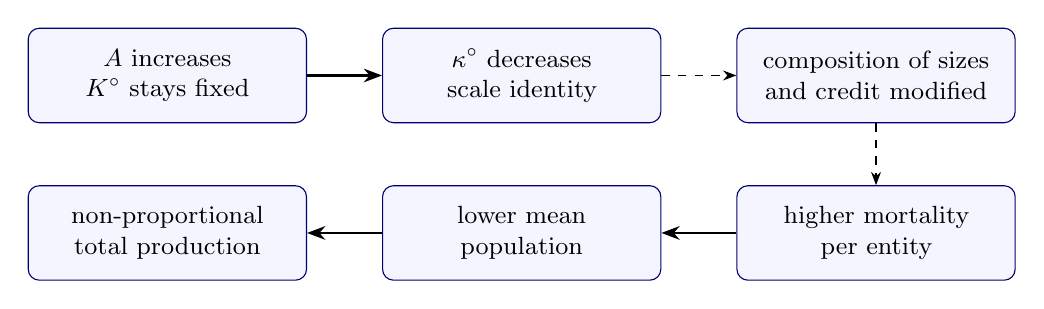
\begin{tikzpicture}[>=Stealth,font=\small,
 box/.style={draw=blue!45!black,fill=blue!4,rounded corners,align=center,text width=3.3cm,minimum height=12mm}]
\node[box] (a) at (0,0) {$A$ increases\\$K^\circ$ stays fixed};
\node[box] (b) at (4.5,0) {$\kappa^\circ$ decreases\\scale identity};
\node[box] (c) at (9,0) {composition of sizes\\and credit modified};
\node[box] (d) at (9,-2) {higher mortality\\per entity};
\node[box] (e) at (4.5,-2) {lower mean\\population};
\node[box] (f) at (0,-2) {non-proportional\\total production};
\draw[->,thick] (a)--(b);
\draw[->,dashed] (b)--(c);
\draw[->,dashed] (c)--(d);
\draw[->,thick] (d)--(e);
\draw[->,thick] (e)--(f);
\end{tikzpicture}
\caption{\textbf{Definitions, measured covariations and proposed
mechanisms.} The first link is algebraic. The dashed links motivate an
interpretation from the paired responses, without isolating a causal
mediation. Under a stable regime, mortality per entity and population
size are linked by the balance of entries and exits; the last step
combines population size with production per entity, which increases.
The solid lines do not therefore all denote an experimentally
identified causality.}
\label{fig:chaine}
\end{figure}

The elasticities of pool dispersion and of credit turnover are
$\ElasticiteGini\pm\ElasticiteGiniIC$ and
$\ElasticiteRotation\pm\ElasticiteRotationIC$ respectively. The
\emph{pool} here denotes the entities drawn for an encounter, not the
whole population; \emph{turnover} is the new principal lent per step
relative to the total stock. Their numerical closeness is a consistency
check, not proof that the first quantity alone causes the second.
Mortality per entity responds with elasticity
$\ElasticiteMortalite\pm\ElasticiteMortaliteIC$; under a stable regime,
it is approximately $\lambda/\overline N$.

Branching provides another measure: under $A\times1.5$ at fixed
endowment, the treated-minus-control contrast of $b_1$ is
$\EffetABranchement$; compensating $K^\circ$ leaves a contrast of
$\EffetResiduelBranchement$. Maintaining $\kappa^\circ$ thus also
brings this statistic closer to the control. The decrease in the
fraction of propagated deaths does not imply a decrease in individual
mortality risk: the two denominators differ.

\subsection{Distributions change with cohorts}\label{sec:ou}
The aggregate does not say where the distributions move. For each
snapshot, we compute the quantiles, then their time average per seed
and finally the treated/control ratio. The figure represents them; the
tabulated values are in Appendix~\ref{sec:tableaux}.

\figurine{art_quantiles}{1.0}{\textbf{Reading positions, not fixed
groups.} M4.4, $A\times1.5$ at fixed endowment, twelve seeds,
$3000<t\le4000$. The abscissa is placed at $\ln[q/(1-q)]$, then graded
in percentiles: the nonlinear scale is explicit and keeps extreme
quantiles legible. Pale points: per-seed ratios; solid points and bars:
mean and 95\% CI. An ordinate of 1.8 means that the considered quantile
is 1.8 times that of the control; it does not mean that the same
entities gained 80\,\%.}

Production shifts by approximately a factor of 1.8; the extreme
quantiles of net worth and gross income increase less than their
medians. The first decile of interest received decreases sharply. The
compositional control confirms the importance of births: among the
10\,\% of entities receiving the least interest, more than 99.9\,\% are
at most ten steps old in the control, against about 24\,\% of the whole
population. Their mean age is about 1.8 steps, against 111 steps for
the whole population. These ages are measured among the survivors of
the main control: $A=1$, $\gamma=1/2$, $\lambda=30$, $K^\circ=25$,
$\delta=\sigma=0.01$, $\rho=1$, $k=2$, free direction and marginal rate.
Over the snapshots from $3010$ to $4000$ spaced ten steps apart, the
mean age is $110.97\pm1.88$ steps, and the average of the instantaneous
medians is $40.05\pm0.16$ steps. Each statistic is first averaged in
time per seed, then across the twelve seeds; the 95\% CIs bear on this
latter average. This is neither the median of a sample pooling all
instants nor the median lifetime. After $A\mapsto1.5A$ on the living
and future entrants from step 2001, with $K^\circ$ unchanged, these two
ages become respectively $94.94\pm0.86$ and $32.03\pm0.24$ steps. A
broader exploration of the amplitudes of variation of $A$ and of values
of $\gamma$ remains necessary for this distributional comparison. The
young-decile diagnostic is specific to the ranking by interest. In the
lowest \emph{capital} decile, the share aged ten steps or less is close
to 49\,\%, not 100\,\%.

\figurine{art_deciles}{1.0}{\textbf{Production, interest and net worth
by capital decile.} M4.4, same arms and window. Entities are reranked
by capital at each snapshot. Reading: the decile-1 point gives the
share of production, interest or net worth held by the 10\,\% least
capital-endowed entities at that instant, not by the same individuals
over 1000 steps. The strong presence of young entities at the bottom of
the ranking contributes to these differences; it is not sufficient to
causally explain the whole profile. Net worth is $NW=K+C-D$; it
replaces stock in the third panel, without changing the ranking
criterion. Groups have equal sizes to within one entity; ties are
broken by stable order. Bars: 95\% CIs across twelve per-seed means,
each computed over the 100 snapshots of the window.}

\section{The credit institution: a complementary lever}\label{sec:partage}
The loan's service allocates the cooperation surplus defined in the
model. Imposing a different share $p$ for the lender changes the
collective state, without changing the technology or introducing new
preferences. This sweep complements the physical steering; it is not
the work's leading result.

\figurine{art_institutions}{1.0}{\textbf{Sharing acts on levels, less on
the balance-sheet Gini.} M4.4, five imposed shares, twelve seeds,
$3000<t\le4000$. Descriptive per-seed linear regressions; mean equations
and $R^2$ shown. Ratios are computed per seed at the $p=0$ arm, whose
raw reference is shown above the panel. The green diamond locates the
historical, so-called archaic, marginal rule at its observed mean
share. It serves only as an illustrative reference, with uncertainty on
both coordinates; it does not enter the regression of the constant
shares. A line between simulated levels is not a validated prediction
at other values of $p$.}

The population goes from about 1904 to 1138 entities as $p$ goes from
zero to one. The reference rule has a mean per-contract share close to
$\PartageParContrat$, but a surplus-weighted share of $\PartagePondere$.
The difference is not a contradiction: small and large surpluses do not
carry the same weight in these averages. The covariance identity and
its proof are given in Appendix~\ref{sec:ponderation}. It does not
establish the causal mechanism of the population change.

Debt relative to production alone does not measure the load ratio on
gross income and does not allow ruling out a convexity of risk in this
load. Appendix~\ref{sec:charge} defines and separately measures the
ratio of interest paid to production \emph{plus interest received}. The
weighting identity does not exempt one from this risk study.

\section{Scope, limitations and next experiments}\label{sec:perspectives}
The model answers a question of existence: can local rules with no
rebound behavior produce a non-proportional aggregate response? In the
configurations studied, yes. It does not yet settle the share of this
mechanism in a real economy. Production added to the stock does not
distinguish primary energy, useful service and final consumption; the
energy rebound in the applied sense \cite{sorrell} requires these
distinctions. The interpretation in terms of exergy entitlements
remains a physical hypothesis, not an empirical calibration.

Distributional plausibility is partial: tails emerge, but their
families are not established, the Gini levels do not simultaneously
reproduce the empirical references, and the "entity" unit is not yet an
identified economic actor. Bankruptcy without recovery, perpetual
principals and the absence of prices are strong hypotheses. The
numerical robustness of the accounts removes none of these limitations.

The SOC hypothesis requires more than a straight-line histogram: it
requires an extended finite-size study, a controlled definition of the
response to a perturbation, and a treatment of memory across steps.
Roots of the intra-step graph may have accumulated fragility in
previous steps. Conversely, merging events close in time can
artificially create a large component. Temporal granularity and the
measurement convention are therefore part of the scientific problem.

The priority extensions are to compare conventions at controlled
$\kappa^\circ$, to jointly study the heterogeneity of
$(K^\circ,A,\gamma)$, and to test a finer-step limit. If $\gamma_i$
varies, the dimension of $A_i$ varies: one must fix a common
$K_{\rm ref}$ and a joint law of
$(K_i^\circ/K_{\rm ref},A_iK_{\rm ref}^{\gamma_i-1},\gamma_i)$, rather
than drawing values of $A_i$ arbitrarily. An exploratory search for a
negative response to an increase in $A$ should state its ranges and
windows in advance, separate the transient from the established
response, and then confirm any identified configuration on new seeds.
No such result is claimed here.

Finally, extending sharing to $p<0$ would have the lender accept a
service initially below its reference productive loss. A later benefit
is possible but not guaranteed; it would depend on trajectories and
bankruptcies. The engine currently imposes $0\le p\le1$ for the fixed
share: this extension remains an experiment to design, not a regime
already simulated.

\section{Conclusion}
The internship's work builds a device for studying the rebound effect
from a physical angle: productive stocks, extraction flows and the
network of commitments evolve together. It brings out collective
regularities that are not imposed, then searches for the parameters
that shift them. Cascade sizes, balance-sheet distributions and
contraction durations do not call for a single statistical family;
distinguishing them is essential to examining the critical hypothesis.

The response to technology constitutes a result of this program: a
uniform individual improvement can produce a sub-proportional
collective increase, because the population and its relative positions
reorganize. The non-dimensional endowment $\kappa^\circ$ makes it
possible to separate two conventions that here lead to different
responses. Time rescaling shows, for its part, that a change of
granularity is not a simple symmetry. These results support the
interest of an organizational explanation of the rebound, while leaving
open the model's criticality and its quantitative confrontation with
the real economy.

\FloatBarrier
\clearpage
\begin{thebibliography}{99}\small
\bibitem{hendrick} M.~Hendrick, A.~Rinaldo and G.~Manoli,
  ``A stochastic theory of urban metabolism'', \emph{PNAS} \textbf{122}(33),
  e2501224122 (2025).
\bibitem{bak} P.~Bak, K.~Chen, J.~A.~Scheinkman and M.~Woodford,
  ``Self-Organized Criticality and Fluctuations in Economics'',
  Santa Fe Institute Working Paper 1992-04-018 (1992).
\bibitem{sorrell} S.~Sorrell and J.~Dimitropoulos,
  ``The rebound effect: Microeconomic definitions, limitations and extensions'',
  \emph{Ecological Economics} \textbf{65}(3), 636--649 (2008).
\bibitem{yakovenko} V.~M.~Yakovenko and J.~B.~Rosser,
  ``Colloquium: Statistical mechanics of money, wealth, and income'',
  \emph{Rev. Mod. Phys.} \textbf{81}, 1703--1725 (2009).
\bibitem{clauset} A.~Clauset, C.~R.~Shalizi and M.~E.~J.~Newman,
  ``Power-Law Distributions in Empirical Data'', \emph{SIAM Review}
  \textbf{51}(4), 661--703 (2009).
\bibitem{herbert} E.~Herbert, G.~Giraud, A.~Louis-Napol\'eon and C.~Goupil,
  ``Macroeconomic Dynamics in a Finite World: the Thermodynamic Potential
  Approach'', \href{https://arxiv.org/abs/2204.02038v2}{arXiv:2204.02038v2} (2022).
\bibitem{wildauer} R.~Wildauer and I.~Heck,
  ``Was Pareto right? Do the US wealth and income distributions follow power
  laws?'', Greenwich Papers in Political Economy, GPERC92, September 2024
  version (series coverage: 2023),
  \href{https://gala.gre.ac.uk/id/eprint/38597/}{institutional archive}.
\bibitem{wright} I.~Wright, ``The duration of recessions follows an
  exponential not a power law'', \emph{Physica A} \textbf{345}, 608--610
  (2005), \href{https://arxiv.org/abs/cond-mat/0311585}{author's text}.
\bibitem{fedgini} A.~Aladangady and A.~Forde, ``Wealth Inequality and the
  Racial Wealth Gap'', \emph{FEDS Notes}, October 22, 2021,
  \href{https://www.federalreserve.gov/econres/notes/feds-notes/wealth-inequality-and-the-racial-wealth-gap-20211022.html}{Federal Reserve}.
\bibitem{cbogini} Congressional Budget Office, \emph{The Distribution of
  Household Income, 2019}, November 2022,
  \href{https://www.cbo.gov/publication/58781}{report and definitions}.
\bibitem{vuong} Q.~H.~Vuong, ``Likelihood Ratio Tests for Model Selection
  and Non-Nested Hypotheses'', \emph{Econometrica} \textbf{57}(2),
  307--333 (1989), \href{https://doi.org/10.2307/1912557}{doi:10.2307/1912557}.
\end{thebibliography}

\noindent\textbf{Reproducibility.} Conventions, point data and sources
are given in the appendices. The author's comments and the previous
version are kept separately, and are not required to compile this
article.
\clearpage
\appendix
\FloatBarrier
\section{Reading glossary}\label{sec:glossaire}
Entries follow the order of first appearance in the body of the
text, after the abstract. Symbols introduced together are grouped;
their operative definitions remain those of the corresponding sections.

\begin{small}
\begin{longtable}{@{}>{\raggedright\arraybackslash}p{.27\linewidth}p{.66\linewidth}@{}}
\toprule Term or notation & Meaning in this article \\
\midrule\endhead
Rebound effect & Deviation from the consumption savings expected after an
efficiency gain. Here, the experiment measures a non-proportional
productive response, without calibrating a final consumption. \\
Endogenous; emergence & Produced by the interactions and evolution of
the system, rather than imposed as a macroscopic target. \\
Self-organized criticality (SOC) & Hypothesis of a regime spontaneously
maintaining itself near a critical threshold. It is not demonstrated
here. \\
Entity & Generic producing agent, able to lend, borrow and disappear;
none of these roles is predefined. \\
$K_i$; productive stock & Mobilizable physical capital of entity $i$,
in model joules; distinct from its net worth. \\
Technology $f_i(K)=A_iK^{\gamma_i}$ & Production added to the stock
during a step; $A_i$ is the extraction coefficient, $\gamma_i$ the
production exponent. \\
$K^\circ$, $\gamma^\circ$ & Birth endowment and production exponent
at birth in the homogeneous reference regime. \\
Principal $q$; service $rq$ & Nominal amount of a loan and interest
due per step; the principal is not amortized. \\
$C_i$, $D_i$, $NW_i$ & Claims, debts and net worth:
$NW_i=K_i+C_i-D_i$. \\
$\lambda$, $\delta$, $\sigma$, $\rho$ & Birth intensity, fraction
depreciated per step, amplitude of the log-normal shock and intensity
of market encounters. \\
Credit institution & Rules fixing the direction, amount and rate of
loans; it does not here designate a particular bank. \\
Invariant; real balance sheet & Relation imposed by the model's
operations. The real balance sheet tracks contributions, production
and stock losses. \\
$B_t$, $\eta_i$ & Number of births at step $t$ and individual
logarithmic shock, renewed at each step. \\
Concavity & Decrease of the marginal return with the stock, for
$0<\gamma<1$; origin of the possible reallocation gain. \\
Service default & Inability to fully pay the interest due at the
step considered. \\
Stock; flow; $\Delta t$ & Quantity held; quantity transferred or
produced during a step; possible physical duration of that step. \\
Exergy & Capacity of a resource to supply work relative to a
reference environment; its correspondence with economic entitlements
remains a hypothesis here. \\
$K_{\rm aut}$, $x_i$ & Deterministic fixed stock of an isolated
entity with no noise or credit; reduced capital $x_i=K_i/K_{\rm aut}$. \\
$\kappa^\circ$, $a$ & Reduced endowment $K^\circ/K_{\rm aut}$;
alternative coefficient $a=A(K^\circ)^{\gamma-1}$. \\
Rescaling; compensation & The former transforms the whole state and
its units; the latter here adapts the endowment of future entrants
to preserve $\kappa^\circ$ after the rise in $A$. \\
Tension $T$; $K_{\rm eq}$ & Ratio $K_{\rm aut}/K_{\rm eq}$; fictitious
stock giving the average production per producer. In the protocols,
$T$ can also denote the horizon of a simulation. \\
$Y$, $N_{\rm prod}$ & Total production of the step and number of
entities present in the productive phase. \\
Marginal return $f'(K)$ & Additional production at the margin per
additional unit of stock. \\
$L$, $\Delta$, $p$ & Productive loss of the lender, joint productive
surplus and share of that surplus attributed to the lender:
$rq=L+p\Delta$. \\
Bankruptcy; cascade; avalanche & Removal of an entity in default or
insolvent; propagation of losses; weakly connected component of
losses among entities that died in the same step. \\
Root; generation; $b_1$, $b_2$ & Initial death; rank of intra-step
propagation; fraction of non-root deaths and average number of
causal links between successive generations per death. \\
Seed; pairing; 95\% CI & Initialization of the random generator;
branches originating from the same state; 95\,\% confidence interval
computed across repetitions, unless stated otherwise. \\
$k$; stationarity & Historical size of the encounter pool, fixed at
two in the main protocol; temporal invariance of statistical
properties, not demonstrated by a single drift test. \\
Little's law & Relation between mean population, arrival flow and
mean lifetime under conditions of stability and boundary control. \\
$S$, $\alpha$, $S_c$, $Z$ & Avalanche size, exponent, exponential
cutoff and normalization constant of its fitted law. \\
Bootstrap; $R^2$ & Resampling of whole realizations; descriptive
goodness-of-fit score, not proof of a family of laws. \\
Contraction; $D$, $\beta$ & Sequence of decreasing steps of a
quantity; duration of that sequence and decay rate of its
exponential survival. $D$ without subscript in this context is not
a debt. \\
Gini; Lorenz & Synthetic inequality index; curve of the cumulative
share of a quantity as a function of the share of entities ranked
by it. \\
Tail; Pareto; log-normal & Domain of large values; power-law
decaying family; family whose logarithm is normal. \\
Finite elasticity $\varepsilon$ & Ratio of the logarithm of the
productive response to the logarithm of the technical factor $m$,
here $m=1.5$. \\
Quantile; decile; cohort & Ranking threshold; group of 10\,\%
reranked at each date; set of individuals tracked by identity. \\
Covariance & Measure of joint variation used in the sharing weighting
identity; it does not demonstrate causality. \\
Load ratio & Interest paid or due, depending on the definition,
relative to production plus interest received; distinct from a
debt-stock-to-production ratio. \\
Vuong & Comparison of model likelihoods on the same sample; its
assumptions and limitations are made explicit in the appendix. \\
\bottomrule
\end{longtable}
\end{small}

\clearpage
\section{Checking the regime studied and the response calculations}\label{sec:stationnarite}
For each seed $s$, arm and observable $X$, we compute
\[
 R_s(X)=\frac{\langle X\rangle_{3750<t\le4000}}
                  {\langle X\rangle_{3000<t\le3250}},\qquad
 t_X=\frac{\overline R(X)-1}{s_R/\sqrt{12}},
\]
where $s_R$ is the standard deviation of the twelve ratios. The 95\% CI is
$\overline R\pm t_{0.975;11}s_R/\sqrt{12}$, with
$t_{0.975;11}\simeq2.201$.
This diagnostic compares two distant temporal levels; it analyzes
neither the full correlation structure nor the stability of the distribution.

\begin{table}[htbp]\centering\small
\caption{Ratio of the means of the last and first 250 steps of the terminal window.}\label{tab:stationnarite}
\begin{tabular}{@{}lrrr@{}}
\toprule
Arm & $R(Y)$ (95\% CI) & $R(N)$ (95\% CI) & $R(\sum K)$ (95\% CI) \\
\midrule
Control & $1.0029\pm0.0152$ & $1.0014\pm0.0132$ & $1.0043\pm0.0178$ \\
$A\times1.5$ & $0.9968\pm0.0139$ & $0.9979\pm0.0116$ & $0.9957\pm0.0167$ \\
$A\times1.5$, compensated endowment & $0.9987\pm0.0132$ & $0.9974\pm0.0122$ & $0.9998\pm0.0148$ \\
Entrants $A\times1.5$ & $1.0088\pm0.0106$ & $1.0070\pm0.0090$ & $1.0092\pm0.0128$ \\
Entrants $A\times0.75$ & $0.9906\pm0.0159$ & $0.9928\pm0.0139$ & $0.9905\pm0.0184$ \\
Entrants $\gamma=0.6$ & $1.0097\pm0.0159$ & $1.0038\pm0.0133$ & $1.0100\pm0.0186$ \\
\bottomrule\end{tabular}\end{table}


None of these contrasts exceeds the usual two-sided threshold, but the
intervals allow drifts on the order of a percent. The temporal observations
of a single run are not used as 1000 independent repetitions.
The result does not automatically hold for an earlier window,
another observable or an unpresented exploratory configuration.

\paragraph{Renewal and memory of the initial state.}
The renewal of a decile provides another time scale, but
the ranking quantity must be specified and the disappearance of an
entity distinguished from its exit from the decile. For a set $D(t_0)$
defined at a reference date, retention
$|D(t_0)\cap D(t_0+h)|/|D(t_0)|$ measures persistence in the group,
while the fraction of its members still alive measures their survival.
These two curves are not interchangeable; the term "first
decile" must specify whether it denotes low or high values.
Even low retention does not demonstrate forgetting of the
initial configuration: commitments and correlations may persist beyond
individuals. This check must be confronted with the autocorrelations of
the observables and with distinct initializations. No quantified
forgetting time is established here; the distance from the final window and
the absence of detected drift are not enough to certify it.

Population balances give exactly
$N(t+1)-N(t)=B(t)-D(t)$ if $B$ and $D$ denote the entries and exits
of the step under the same counting convention. Over a long stable window,
$\overline B\simeq\overline D$ and $\overline B\simeq\lambda$;
the ratio $\overline D/\overline N$ becomes close to
$\lambda/\overline N$. This is not exactly the mean of
$D(t)/N(t)$, and boundary terms are not zero by decree.
The relation explains why a mortality elasticity can be
almost the opposite of a population elasticity without constituting an
independent causal finding.

The elasticity of equation~\eqref{eq:eps} concerns a finite
intervention. Its mean and CI are computed after forming the twelve
paired log-ratios, not after averaging all time points
in both arms. The decomposition formulas are sensitive to the
choice of population: entities present at production may
disappear before the end-of-step snapshot. This difference is
preserved in the source data; it must not be erased to
force the numerical closure of an ill-defined identity.

\section{Distribution fits: definitions and limitations}\label{sec:ajustements}
\subsection{Mass, per-bin density and survival function}
For an integer size $S$, the mass $P(S=s)$ and the survival
$P(S\ge s)$ are distinct. The histogram here represents the mass
of a bin $[l,r[$ divided by $r-l$, so that a wide bin does not
appear more probable merely because it contains more
sizes. The fitted curve is summed over the same integer sizes
before this division. A survival slope cannot be
substituted directly for the mass exponent.

The descriptive likelihood of the law~\eqref{eq:avalanche} is maximized
per seed, over all sizes $s\ge1$. The numerical normalization
uses $1\le s\le20000$; the mass of the last thousand values is
checked to be below $10^{-10}$ at the optimum. The numerical search
bounds are $-2\le\alpha\le5$ and
$10^{-5}\le1/S_c\le2$; an optimum at a bound would signal
insufficient identification. The 24 fits presented are interior.
The fitting support is not chosen to maximize the apparent
straightness of a subset of points.

The cross-seed CIs and the bootstrap over whole runs measure the
variability of the estimators or of the average curves obtained by this
protocol. Fitting by product of probabilities does not demonstrate
the independence of a run's avalanches. We therefore do not derive
event-level standard errors or a certified goodness-of-fit test from it.
In particular, this should be complemented by a comparison of families on
the same support and an absolute-adequacy diagnostic accounting
for temporal dependence \cite{clauset}.

The descriptive coefficient shown is
\[
 R^2_{\log}=1-
 \frac{\sum_j[\log\widehat p_j-\log p_{j,\rm fit}]^2}
      {\sum_j[\log\widehat p_j-\overline{\log\widehat p}]^2},
\]
over the non-empty empirical bins. This is not a percentage
of correctly predicted probability, and it is not the criterion
optimized by the likelihood. It depends on the binning. Zeros are
not replaced by an arbitrary small value to make them
loggable.

\subsection{Durations: discrete exponential and window choice}
If $D\ge1$ follows a geometric law, with stopping probability $u$ at
each step, then $P(D\ge d)=(1-u)^{d-1}$ and
$\widehat u=1/\overline D$. Thus
$\widehat\beta=-\log(1-1/\overline D)$ in
$P(D\ge d)=\exp[-\beta(d-1)]$.
The regressions of figure~\ref{fig:art_cycles} use this
normalized form, not a log-log line. The $R^2$ there is computed
on the non-zero log-survivals, at durations 1 to 11. Episodes remain
potentially correlated and the window boundaries truncate some
of them; the CIs are therefore based on the five seeds and not on
a fictitious number of independent recessions.

\subsection{The Vuong test and what it actually compares}
In the existing analyses of net worth and interest, the threshold
$x_{\min}$ is chosen by minimizing a Kolmogorov--Smirnov
distance for a continuous power law. Above this same
threshold and on the same values, a log-normal and an
exponential are also fitted, conditioned on $X\ge x_{\min}$.
The power law compared here has \emph{no upper cutoff}: this
is not the discrete model with exponential cutoff used for avalanches.
The \emph{left} truncation, which defines a tail sample,
must not be confused with the \emph{right} cutoff.

For the fitted densities $f$ and $g$, define
$d_i=\log f(x_i)-\log g(x_i)$ and then
\[
 z=\frac{\sqrt n\,\overline d}{s_d},\qquad
 s_d^2=\frac1{n-1}\sum_i(d_i-\overline d)^2.
\]
A positive value favors $f$ in average log-likelihood.
The usual interpretation of $\pm1.96$ as a 5\%
threshold requires regularity, model-separation
and sampling assumptions. Here the threshold was selected, entities
interact, and some fitted log-normals are very close
to a power-law limit. The score is therefore reported as a diagnostic,
not as certification of these assumptions \cite{vuong}.

The flag $\sigma_{\rm LN}>10$ concerns 50 of the 72 interest
fits and 46 of the 72 net-worth fits. It marks a
numerical zone, not a mathematical boundary between two families.
Two visible groups in a scatter of fit parameters do not
mean that the agents form two economic populations:
each point in that scatter represented one fit, not one entity.
Per-fit results and their identifiers are available in
\chemin{data_revision/rev_vuong_points.csv}.

Comparing Pareto, cutoff power law and log-normal requires
fixing the same domain, describing the threshold selection and evaluating
goodness of fit, not merely counting parameters. A cutoff
that diverged with system size would define an interesting
limit, to be checked across several sizes; it does not make
its finite-size fit free of charge.

\section{Credit load and surplus weighting}
\subsection{Definition and measurement of the load ratio}\label{sec:charge}
Let $P_i$ denote the step's production, $I_i^{\text{received}}$ the interest
received, $I_i^{\text{paid}}$ that actually paid, and $D_i$ the
sum of principals due. Three ratios must be distinguished:
\[
 c_i^{\text{paid}}=\frac{I_i^{\text{paid}}}{P_i+I_i^{\text{received}}},\qquad
 c_i^{\text{due}}=\frac{\sum_{\ell:i\,\mathrm{borrows}}r_\ell q_\ell}
                         {P_i+I_i^{\text{received}}},\qquad
 d_i^{\text{income}}=\frac{D_i}{P_i+I_i^{\text{received}}}.
\]
The first is a share of gross income paid; the second is the
contractual charge due; the third relates a debt stock
to a per-step income and is interpreted in a number of steps. The
variable $D_i/P_i$ represents neither of the first two ratios.
The denominator includes financial income, even though its
aggregate sum is not new real production.

\figurine{art_charge}{0.95}{\textbf{A correctly named load
diagnostic.} Marginal rule M4.4, twelve seeds. For the snapshots
$3000<t\le3990$, the variable is
$I_i^{\text{paid}}/(P_i+I_i^{\text{received}})$; the response is the fraction
of entities dying in the following ten steps. The bins have the
explicit bounds shown, common to all seeds; they are
not capital classes. The last incomplete window is
excluded. The 95\% CIs compare the fractions obtained across twelve runs,
without attributing binomial independence to repeated entities.
All-cause deaths and insolvency roots are shown separately.}

The panels record the interest paid, not the service due
at the exact moment preceding payment. A pro-rata payment can
make an unsustainable load look low; the moment of
collection and the flows received within the step also matter.
The diagram remains descriptive, conditional on the survivors observed
in the panel. It justifies neither a causal link from load to
death nor a general refutation of convexity. Convexity
calculations or Jensen-gap computations on $D_i/P_i$ would not answer
the question asked here about the load ratio as defined.

\subsection{Proof of the weighting identity}\label{sec:ponderation}
For $n$ contracts whose mean surplus is strictly positive,
let $\overline p=n^{-1}\sum p_j$,
$\overline\Delta=n^{-1}\sum\Delta_j$ and
$p_w=\sum p_j\Delta_j/\sum\Delta_j$.
Defining the empirical covariance with denominator $n$,
\[
 \operatorname{Cov}_n(p,\Delta)
 =\frac1n\sum_j(p_j-\overline p)(\Delta_j-\overline\Delta)
 =\frac1n\sum_jp_j\Delta_j-\overline p\,\overline\Delta,
\]
we immediately obtain
\begin{equation}
 p_w-\overline p=\frac{\operatorname{Cov}_n(p,\Delta)}{\overline\Delta}.
 \label{eq:identite}
\end{equation}
If a corrected covariance with denominator $n-1$ is used,
the numerator must be multiplied by $(n-1)/n$. The identity also
holds in expectation when the moments exist and
$\mathbb E[\Delta]\ne0$.

For a constant fixed sharing rule, the gap is zero by construction.
For a variable rule, it can be positive even if most
contracts have a very small principal or surplus. The
effective distribution of contracts determines its magnitude; an
analytical grid covering rarely realized contracts cannot
replace this distribution. Qualifying a rule from
these theoretical cases alone would overstate their empirical reach.
The accounting identity does not demonstrate an explanation of
mortality or population differences between institutions.

\section{Measurement supplements and tabulated values}\label{sec:tableaux}
\subsection{Quantile ratios}
The table below and figure~\ref{fig:art_quantiles} rest
on the same observations. Each $\pm$ is a half 95\% Student CI
of the twelve per-seed ratios, not a standard deviation across
entities. "Gross income" means production plus interest received.
\begin{small}\input{table_quantiles_en}\end{small}

\subsection{Temporary reach of an intervention}
An intervention limited to the entities present can die out
with their cohort if entrants do not inherit it. This
partial-reach experiment is a protocol control,
not a main proof of the rebound mechanism. Conversely,
modifying all entities and future entrants preserves
the treatment despite population renewal. Modifying
$\gamma$ changes the shape of the function and the dimensions of
its coefficient: this is not the same operation as multiplying
$A$ at fixed $\gamma$.

\subsection{Multiple losses and sufficient causes}
The graph can attribute several losses to a victim.
This does not mean that each would have sufficed, in isolation, to
make it insolvent. To illustrate this, an initial net worth
of 5 and two losses of 3 lead to $-1$; no single loss
suffices. With a net worth of 2, each of the two losses
would suffice. It is the solvency margin before the losses that
makes the difference, not merely the number of edges.

The count of parents must also specify whether it retains only
losses coming from the previous generation or all
those of the step. A detailed sufficiency analysis also requires
reconstructing the debts written off; it is not
necessary to establish the existence of propagation nor the
non-proportionality of the response. Earlier calculations
remain archived, but their percentages are not used
as evidence in this article.

\subsection{Stock and production on the same realization}
\figurine{rev_stock_trajectoire}{0.95}{\textbf{Observing the difference between
stock and flow.} M4B central, seed 11, excerpt $3000<t\le3200$.
Each line follows a single realization, with no measurement
uncertainty artificially added; the orange points mark
the down-steps. The contraction durations are computed separately
on the two observables in figure~\ref{fig:art_cycles}.}

\FloatBarrier
\section{Local sources, configurations and reproducibility}\label{sec:sources_revision}
The PDF can be compiled with only the LaTeX files and figures
in this folder, without the internship report or the questionnaires.
The new calculations are produced by
\chemin{../scripts/revision_article.py}, which writes only into
this article's folder and launches no simulation.
The numerical exports, per-seed observations and
SHA-256 checksums of the sources are in \chemin{data_article/}.
The retained supplements from the previous version are in
\chemin{data_revision/}. Recomputing from the microdata
requires the local campaigns, which are not all version-controlled.

\subsection{Three protocols, samples not merged}
\begin{small}
\begin{longtable}{@{}p{.18\linewidth}p{.75\linewidth}@{}}
\toprule Family & Configuration and data \\\midrule\endhead
M4B central & $A=1$, $\gamma=1/2$, $\lambda=30$, $\delta=0.05$,
$\sigma=0.25$, $K^\circ=25$, $k=3$, geometric target. Five seeds
11--15; contractions on $1000<t\le4000$, Gini on the final state.
Simulation Lab identifiers are in the episode and confirmation
exports. The Gini sweep shown varies $\sigma$ only. \\
Live-v1 recalibration & Reference $A=1$, $\gamma=1/2$, $\lambda=30$,
$\delta=\sigma=0.01$, $K^\circ=25$, $\rho=1$; seeds 0--2,
empty start. Window $1200<t_{\rm old}\le2000$.
The fine-depreciation arm uses its own reference $\delta=0.002$.
The folders are named in \texttt{temps\_graines.csv}. \\
M4.4 main & Same physical reference as Live-v1; arithmetic target
in the homogeneous regime, free loan direction, marginal rule. Twelve seeds
0--11, intervention at step 2001, window $3000<t\le4000$.
Compensated endowment: $K^\circ=56.25$ for new entrants
after the intervention; existing stocks unchanged. \\
M4.4 sharing & $p\in\{0;0.25;0.5;0.75;1\}$ or marginal rule;
twelve seeds, same window. Ratios to the $p=0$ arm are paired.
Load diagnostic: marginal rule only, $3000<t\le3990$,
ten-step death horizon. \\
M4.4 encounters & $\rho\in\{0.5;1;1.5;2;3\}$; twelve seeds
per value. Balance-sheet Ginis are recomputed on the panels of
$3000<t\le4000$, like the windows of the other measurements. \\
\bottomrule
\end{longtable}
\end{small}

\subsection{Each figure and its data-point files}
The CSV files with no prefix and \chemin{diagnostic_chaine.json} are
relative to \chemin{data_article/}. The TeX files and paths
starting with \chemin{data_revision/} are relative to the LaTeX folder.
The manifest links the exports to the original
sources and their checksums; it does not turn an aggregated export
into complete microdata.
\begin{footnotesize}
\begin{longtable}{@{}p{.09\linewidth}p{.48\linewidth}p{.36\linewidth}@{}}
\toprule Fig. & Data / local file & Nature of the calculation \\
\midrule\endhead
\ref{fig:exemple} & \chemin{exemple_article.tex} & Four fictitious entities,
real loan and nominal recording; no simulated measurement. \\
\ref{fig:art_technologie} & \chemin{technologie_points.csv},
\chemin{technologie_courbes_v2.csv} & Analytical technologies
$2K^{1/4}$ and $K^{1/2}$; no regression. \\
\ref{fig:cascade} & \chemin{cascade_article.tex} & Fictitious five-entity
balance sheet; four-bankruptcy tree checked separately. \\
\ref{fig:art_avalanches} & \chemin{avalanches_counts.csv},
\chemin{avalanches_fits.csv}, \chemin{avalanches_points.csv} & Integer
sizes in the avalanche CSVs; fits and cross-seed CIs. \\
\ref{fig:art_cycles} & \chemin{cycles_fits.csv}, \chemin{cycles_points.csv};
episodes in \chemin{data_revision/rev_cycles_episodes.csv} & Five
M4B runs; exponential coefficient from the mean duration. \\
\ref{fig:art_lorenz} & \chemin{lorenz_points.csv}, \chemin{lorenz_ginis.csv} &
Control panels; exact dates 2010, 3000, 4000. \\
\ref{fig:art_sensibilite} & \chemin{m4b_sensibilite_points.csv},
\chemin{m4b_nw_confirmation.csv} & NW Gini on five independent final
snapshots per cell. \\
\ref{fig:art_rho} & \chemin{rho_points.csv}, \chemin{rho_fits.csv},
\chemin{rho_nw_graines.csv} & Three estimators from the campaign table,
plus recomputed NW Gini; per-seed regressions. \\
\ref{fig:art_temps} & \chemin{temps_graines.csv}, \chemin{temps_points.csv} &
Live-v1 series rescaled to a common duration and a common flow per
old step. \\
\ref{fig:art_reponse} & \chemin{elasticites_graines.csv}; curves in
\chemin{data_revision/rev_reponse_courbes.csv} & Elasticities recomputed
from the series; centered 101-step smoothing kept for the curves. \\
\ref{fig:chaine} & \chemin{corps_article.tex}; diagnostics
\chemin{diagnostic_chaine.json} & Interpretive diagram,
not a causal graph identified by intervention on each mediator. \\
\ref{fig:art_quantiles} & \chemin{data_revision/rev_quantiles_graines.csv} &
Per-seed ratios kept; abscissa transformed to logit. \\
\ref{fig:art_deciles} & \chemin{deciles_v2_points.csv},
\chemin{deciles_v2_graines.csv} & Shares of production, interest and NW;
ranked by capital at each snapshot. \\
\ref{fig:art_institutions} & \chemin{institutions_points.csv},
\chemin{institutions_fits.csv}, \chemin{institutions_references.csv} &
Ratios to $p=0$ and descriptive linear regressions. \\
\ref{fig:art_charge} & \chemin{charge_graines.csv}, \chemin{charge_points.csv},
\chemin{charge_resume.csv} & Interest paid / gross income; deaths
observable throughout the horizon. \\
\ref{fig:rev_stock_trajectoire} &
\chemin{data_revision/rev_stock_trajectoire_points.csv} &
Raw M4B excerpt; figure kept. \\
\bottomrule
\end{longtable}
\end{footnotesize}

The new age-composition checks are in
\chemin{ages_graines.csv}. The ranking conventions are
explicit in the script; ties are broken by stable order. The revision
plan and the decision register are outside the LaTeX folder, in
\chemin{../revision_2026-09-15/}, to keep the corrections to be
reported in the internship report separate.

The supplement on instantaneous median ages is computed by
\chemin{../scripts/ages_v2.py}. Its per-seed values, its averaging
convention and the checksums of the source panels are kept in
\chemin{../revision_2026-09-17/ages_v2_graines.csv} and
\chemin{../revision_2026-09-17/ages_v2.json}. It runs no
simulation and modifies no figure generator.


The detailed configurations and the M4.4 identifiers of the
initial campaign remain in
\chemin{data_revision/runs_m44.csv}, which distinguishes the
recorded parameters from the interventions. Some seeding metadata
does not record the parameters; these gaps are not filled
by silent deduction.
The technical \texttt{K0} codes from the source files are
kept for their traceability; in the scientific notation,
the endowment is now read $K^\circ$ and its reduced ratio
$\kappa^\circ$. Renaming the notation does not modify the engines.

\subsection{Engine compatibility and rule changes}
\label{sec:compatibilite}
Three levels of control must be distinguished: preserving the
functionalities of the simulation lab, reproducing a trajectory
in a reference regime, and comparing two models whose rules
differ. Only the second bears directly on dynamic parity.

The M4.2 report, section "M4B Parity", documents tests at
$A=1$, $\gamma=1/2$ and $k=2$: identity of discrete variables
and comparison of floats at relative tolerance $10^{-9}$.
The reported 1000-step probe shows no discrete divergence,
with a maximum relative deviation of the series of $3.1\,10^{-12}$.
This finding is not a bit-for-bit identity nor a guarantee at every horizon.

For M4.4, in the campaign folder
\chemin{m4_4_rebond_credit_soc/}, the file
\chemin{results/analysis/parity_deviations_8000.csv}
holds 8000 maximum deviations, all zero, over the 26 columns compared to
the reference M4.3 run, in the homogeneous regime with arithmetic
target. The test \chemin{tests/test_parity_m4_3.py} defines this
scope. The test \chemin{tests/test_v1_equivalence.py} separately compares
Live-v1 to the compatibility mode
\texttt{richest\_lends}, with a heterogeneous intervention; a negative
control checks that freeing the loan direction can change the trajectory.
The presence of this test defines a verifiable requirement; it does not by
itself replace an execution report for every version.

The M4.4 campaign paths are kept as provenance identifiers. Switching
to a different market rule must be distinguished from an instrumentation
extension, without renaming the archives the data come from. Non-regression
therefore does not allow merging the M4B, Live and M4.4 samples.

\subsection{Why temporal aggregation is not a symmetry}
\label{sec:composition_temps}
A counterexample appears even before introducing the market. With no noise,
credit or births, let $F(K)=(1-\delta)(K+AK^\gamma)$.
Two successive steps give
\[
F(F(K))=(1-\delta)^2(K+AK^\gamma)
 +(1-\delta)A\big[(1-\delta)(K+AK^\gamma)\big]^\gamma.
\]
An aggregated step, with $A'=2A$ and
$1-\delta'=(1-\delta)^2$, would instead give
\[
G(K)=(1-\delta)^2(K+2AK^\gamma).
\]
In general $F\circ F\ne G$: the second production is computed on
an already modified stock. For example, at $K=100$, $A=1$,
$\gamma=1/2$ and $\delta=0.01$, the values are approximately
$118.142$ and $117.612$. The market adds an alternation of
encounters, contracts, interest and bankruptcies; composing the Poisson
laws or the shocks alone does not compose these coupled operations.

The Live-v1 trials of figure~\ref{fig:art_temps} measure the collective
reach of this difference. After full conversion of the parameters,
aggregating two steps gives, relative to its reference,
$N:1.067\pm0.018$, $K_{\rm tot}:1.158\pm0.030$ and
$Y:1.118\pm0.024$. Aggregating four steps, the production ratio
is $1.346\pm0.026$. The protocol starts from an empty state,
uses three seeds and compares $1200<t_{\rm old}\le2000$;
flows are divided by the aggregation factor, not the stocks.
The per-seed values and other variants are in
\chemin{data_article/temps_graines.csv} and
\chemin{data_article/temps_points.csv}. These trials and the counterexample
establish the absence of an exact symmetry; they do not constitute
a study of convergence toward a continuous limit.


\end{document}
